\chapter{Prototypen} 

I dette kapittelet vil det bli gitt en innføring i valg som ble tatt før og underveis i utviklingsprosessen. 
 
\section{Utgangspunkt} 
\label{sec:utgangspunkt} 

Målet med forskningen var å undersøke potensielle forbedringer funksjonene beskrevet i seksjon \ref{sec:ResearchQuestion} kunne ha på programvaren Sono Flex. Det mest naturlige valget ville da  ha vært å implementert de ønskede funksjonene i den eksisterende koden. Tobii Dynavox ønsket derimot å utforske andre muligheter. Blant annet fordi den eksisterende teknologien hadde flere begrensninger som ville gjort det vanskelig å fått implementert mye av funksjonalitet som skulle undersøkes. Spesielt gjelder dette animasjonene. Resultatet ble at utviklingen ble startet som et nytt prosjekt og at første del ble å lage en high-fidelity prototype ved å bruke "reverse engineering" på Sono Flex.


\section{Kravspesifikasjon} 

Å implementere all funksjonaliteten som Sono Flex har, ville vært for ressurskrevende. Det ble heller bestemt å fokusere på det mest nødvendige og heller gjøre dette skikkelig. Slik at det var mulig å bygge videre på koden i ettertid. Det mest nødvendig vil si hoved funksjonaliteten, som er å la en bruker ha mulighet til å skrive setninger med symboler for så å gjøre om disse til naturlig tale. For å kunne gjennomføre dette er det flere mindre oppgaver som måtte implementeres. 

-	Mulighet for parter som ikke deltok i prosjektet å videreutvikle koden.
-	Den må være koblet til 

Under er kravspesifikasjonen. De ulike kravene er beskrevet etter prioritert, der de første er de mest nødvendige og kjent som kjernefunksjonalitet. Deretter vil funksjonalitet som hadde vært greit å ha, men som ikke er nødvendig for at applikasjonen skal kjøre, beskrevet.  
 
\subsection{Funksjonelle krav} 
 
 
\textbf{Øyesporing som interaksjon} - Det skal være mulig å bruke \underline{kun} øyene til å operere prototypen. En som tar i bruk øyesporing skal ha akkurat de samme mulighetene som han ville hatt ved å ta i bruk datamus. Effektiviteten skal være så lik som mulig mellom de to interaksjonsformene. 
 
\textbf{Logging} - I systemet skal det være mulig å kunne logge all interaksjonen en bruker gjør med programvaren. Denne funksjonen vil være nødvendig for å kunne gjennomføre testingen 
 
\textbf{Brukertilpasning} - Hver bruker skal ha mulighet til å kunne tilpasse programvaren etter sine preferanser. 
  
\textbf{Tale} - Systemet skal kunne gjøre om tekst til lyd. Det vil si at andre personer skal kunne forstå setningen brukeren har skrevet kun utifra lyden. Jo mer naturlig talen høres ut jo bedre.
  
\textbf{Norsk} - Systemet skal ha språkstøtte for norsk. Bør også legges opp til mulighet for å endre og legge til støtte for andre språk 
 
\textbf{Animasjon} - I prototypen skal det være animasjoner som blir aktivert når en bruker trykker på de ulike symbolene.  

\textbf{Lydeffekter} - Utenom talelyden, skal det også være lydeffekter som skal avspilles ved brukerinteraksjon.  
 
\textbf{Symbol} - For vært ord skal det være symbol som representerer ordet. En bruker skal i teorien, ikke ha behov for å lese ordet og skal kun i utifra ordet forstå hvilket ordet det representerer. 


 
\subsection{Ikke-funksjonelle krav} 
 
\textbf{Brukervennlighet} - Målgruppen består av barn med som har begrenset erfaring med å operere dataprogrammer. Det er derfor viktig at det legges vekt på det og programvaren utformes på en måte som er intuitiv for brukeren.   
 
\textbf{Fleksibilitet} - Kodebasen skal være tilrettelagt for vedlikehold og videreutvikling. Det er viktig at personer som ikke har deltatt i systemutvikling skal ha mulighet til å forstå koden og på den måten enkelt kan legge til og fikse funksjoner. Programvaren skal også legge oppp til at det er enkelt og legge til animasjoner, lyd og nye brikker. 
 
 \textbf{Responstid} -  Programvaren er kompleks og det tar lang tid å skrive med symboler, det er derfor viktig at systemet responderer kjapt og ikke gjør slik at oppgaven tar lenger tid. Slik at når brukeren trykker på noe skal det føles som om programvaren svarer momentant. 

\textbf{Personvern} - Brukerne av programvaren er en sårbar gruppe, det vil derfor være viktig at sensitiv informasjon om disse ikke kommer på avveie. Det skal i utgangspunktet ikke lagres sensitiv data, men hvis data lagres skal det lagres på en sikker måte. 
 
\section{Utvikling} 
 
I denne seksjonen vil teknologier og arbeidsområde bli beskrevet, som skal gi grunnlag for den neste seksjonen som vil gå mer innpå implementasjon valg og detaljer. 
 
 
\section{Programmeringsrammeverk} 

Programmeringsrammeverk er ikke nødvendig for å kunne bygge prototypen, men tilbyr flere gode fordeler. Blant annet lav-nivå kode som allerede har blitt bygget, testet og som har blitt brukt av andre programmerere, noe som øker påliteligheten og reduserer utviklingstiden \cite{Frame7:online}.

Til å utvikle prototypen ble det brukt .NET. Dette kom som et resultat av at
to faktorer. Den en var dokumentasjonen til øyesporingsenheten anbefaler det og alle eksemplene av bruk er i en .NET teknologi. Den andre var at rammeverket tilbyr flere gode brukergrensesnitt-teknologier som var ønskelig med tanke på at brorparten av utviklingen handler om det grafiske.


\subsection{.NET}
 
Arkitekturen til .NET er omfattende og som en kan se utfra figur \ref{fig:net-arkitektur} er det flere programmeringsspråk og komponenter en kan velge å ta i bruk. Rapporten vil derimot kun gi informasjon om de ulike komponentene fra .NET som ble brukt og er nødvendig for videre lesning. 
 
 
\begin{figure}[ht] 
\centering 
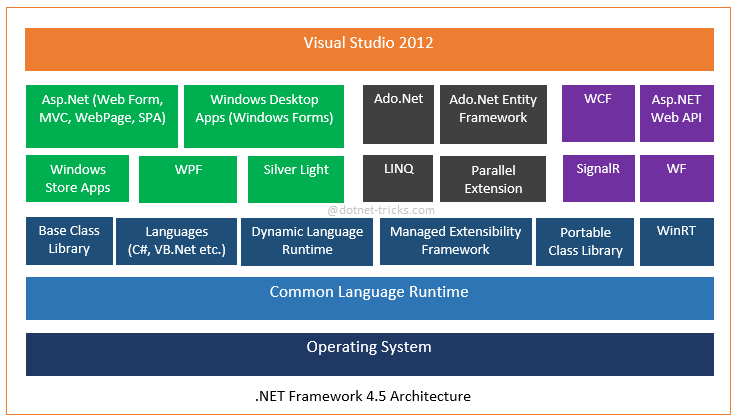
\includegraphics[width=140mm]{netframework45} 
\caption{Diagram som viser arkitekturen til .net rammeverket versjon 4.5} 
\label{fig:net-arkitektur} 
\end{figure} 
 
 
\section{Brukergrensesnitt-teknologi} 

Brukergrensesnitt-teknologi gir utvikleren tilgang på funksjoner og forhåndsdefinerte grafiske elementer som skal gjør utviklingen mer effektiv. Som en kan se utifra figur \ref{fig:net-arkitektur} og Microsoft's oversikt \cite{User1111:online} tilbyr .NET teknologier som Windows Store Apps, Windows Presentation Foundation(\gls{WPF}), Expression Blend 3 + SketchFlow, Windows Forms og Silverlight. Alle disse ble evaluert før et endelig valg ble foretatt:

\textbf{Windows Forms} ble utelukket ettersom dette er teknologien som Sono Flex er bygget på og som hadde begrensinger som gjorde at flere ønskede funksjoner ble vanskelig å implementere. 

\textbf{Windows Store Apps} hadde mye av den ønskede funksjonaliteten, samtidig som den fortsatt vedlikeholdes. Problemet var at for å distribuere slike applikasjoner brukes Windows Store. F å få publisert applikasjonen der, kreves godkjenning av Windows. En tidkrevende prosess. Dette i sammenheng med at disse applikasjonene ikke er kompatible med Windows 7\cite{Windo0:online} gjorde at denne teknologien ikke ble valgt. 

\textbf{Silverlight} er ifølge Microsoft sin blogg\cite{User1111:online} en kraftig utviklingsplattform for å lage "rike" media- og forretningsapplikasjoner for web, skrivebord og mobil. Fokus for teknologien er derimot på web og mobil \cite{Micro6:online}, og ettersom prototypen er en skrivebords applikasjon falt ikke valget på Silverlight.

Teknologien som til slutt ble valgt var \textbf{Windows Presentation Foundation}. WPF skal tilby utviklere en helhetlig programmeringsmodell for å bygge skrivebordsapplikasjoner for Windows som tar i brukergrensesnitt, media og dokumenter \cite{Windo777:online}. Grunnen til at teknologien ble valgt er:


\begin{itemize}
\item Fokus på skrivebord. I motsetning til blant annet Silverlight, er WPF designet og laget for å utvikle klient applikasjoner\cite{Windo777:online}.
\item Prioritert av Tobii PC Eye GO. I dokumentasjonen til øyesporingsenheten er det skrevet: "WPF  rammeverket er et svært bra verktøy for utvikling av grafikk-intensive applikasjoner og WPF har derfor blitt gitt høyest prioritet [..]"
\item Etterfølgeren til Windows Forms . Er ifølge Microsoft erstatteren til teknologien som blir brukt i Sono Flex \cite{User1111:online}. 
\item God støtte for animasjoner. WPF tilbyr blant annet et eget timing system for å enkelt holde tiden når en animerer grafiske elementer \cite{Anima7:online}.
\end{itemize}



 
\subsection{Windows Presentation Foundation} 
 
Ifølge Adam Nathan \cite[p.~9]{WPFbook}, programvare arkitekt hos Microsoft, ble prosessen med å lage WPF igangsatt fordi at mens grafisk maskinvare hele tiden har blitt bedre og billigere - samt at forbrukerens forventninger har fortsatt å stige, så var ingen som hadde adressert vanskeligheten med å lage moderne brukergrensesnitt.  

Han argumenterer med at det fantes utviklere på tiden som for eksempel brukte bitmap bilder til for å få et et annet utseende på for eksempel knappene enn det standardknappene hadde. Problemet er at disse formene for tilpasning ikke bare kan være ressurskrevende å utvikle, men også gi en dårligere brukeropplevelse. 

Han forteller videre at de ønsket å lage et rammeverk som hadde produktiviteten som folk likte med Windows Forms og som var enkel som HTML og Javascript.

WPF gir utvikleren mulighet til å utvikle applikasjoner med å bruke både markup språk og kode. Markup språket brukes vanligvis til å implementere utseende til applikasjonen, mens programmeringspråket brukes vanligvis til å implementere oppførselen. Det vil si at det er mulig å bruke de på tvers, men WPF legger opp til å skille mellom utseende og oppførsel \cite{Intro8:online}. Dette skillet skal ifølge utviklerene gi flere fordeler som blant annet reduksjon av utvikling og vedlikeholdskostnader ettersom utseende-spesifikk markup ikke er tett koblet med oppførsel-spesifikk kode. Det gir også designere mulighet til å jobbe med utseende samtidig som utviklere jobber med oppførsel \cite{Intro8:online}. I WPF er eXtensible Application Markup Language (XAML) brukt som markup språk. Mens man som programmeringspråk kan velge mellom C-Sharp eller Visual Basic.

\subsubsection{C-Sharp} 

Valget av programmeringsspråk sto mellom C-Sharp og Visual Basic (VB), to språk med svært forskjellig syntaks og historie \cite{Compa6:online}. C# har basert syntaksen sin på programmeringsspråket C , mens VB har sine røtter fra programmeringspråket BASIC \cite{Visua3:online} \cite{About8:online}. Begge språkene har de samme mulighetene, forskjellen ligger hovedsaklig i syntaks, så valget av programmeringsspråk ble basert på preferanser \cite{What0:online}. I dette tilfelle ble det valgt å ta i bruk C-Sharp, mye på grunn av likheten med Java som vi hadde erfaring med fra tidligere, men også på grunn dette var språket som ble mest brukt i eksempler og i dokumentasjonen til øyesporingenheten.


\subsubsection{eXtensible Application Markup Language (XAML)} 

XAML, en dialekt av XML, og har vært en viktig del av WPF siden dens introduksjonen i 2006 \cite[p.~17]{WPFbook}. Vanligvis brukes XAML til å spesifisere brukeregrensesnitt objekter og organiseringen av dem, men kan også brukes til andre ting som for eksempel animasjoner \cite{Story5:online}. 

Grunnen til at XAML har blitt brukt er fordi det er enkelt for programmere å samarbeide med eksperter fra andre felt. Nathan forteller at XAML blir felles språket for alle partiene, hovedsaklig gjennom utviklingsverktøy og felt-spesifikke design verktøy. Men også fordi XAML (og XML generelt) er enkelt å lese og forstå \cite[p.~17]{WPFbook}. Figur \ref{listing:knapp} viser hvor enkelt en kan genere en blå knapp som også er lettleselig .


\begin{listing}[ht] 
\inputminted[fontsize=\footnotesize, frame=lines,framesep=2mm,baselinestretch=1.2,bgcolor=lightgray,linenos]{xml}{Code/xamlexample.xml} 
\caption{Hvordan en blå knapp blir definert i XAML} 
\label{listing:knapp} 
\end{listing} 
 
   
\section{IDE og versjonskontroll} 

For å automatisere mye av utviklingen ble det valgt å bruke utviklingsmiljøet Visual Studio 2013 \cite{2013-1:online}. Grunnen til at Visual Studio ble valgt er det for at i tillegg til å ha kode-redigeringsverktøy og debugger, så har den også en WPF designer\cite{What8:online}. Denne designeren tilbyr flere hjelpemidler for å effektivisere prosessen med å lage brukergrensesnitt. Blant annet kan man velge mellom å kode de forskjellige elementene eller man kan dra dem inn fra et sidepanel. Den viktigste er derimot design vinduet, som til enhver tid viser hvordan brukergrensesnitt blir uten å måtte kjøre koden\cite{WPF D1:online}. 
 
For versjonskontroll ble det på grunn av erfaringsmessige årsaker brukt git\cite{AboutGit:online}. Til å ta backup av git filene ble den web-baserte tjenesten Bitbucket brukt. Grunnen til dette var at mye av koden fra Tobii Dynavox var konfidensiell og Bitbucket tilbyr gratis hemmelig oppbevaring. 
 
 
\section{Model View ViewModel} 

En viktig del av oppgaven var å bygge en prototype som Tobii Dynavox kunne bygge og teste videre på. Det var derfor en forutsetning at kildekoden var tilrettelagt for vedlikehold og videreutvikling. For å gjennomføre dette valgte vi å følge arkitekt mønsteret Model view Viewmodel (MVVM). Grunnen til at vi valgte dette fremfor mønster som for eksempel Model View Contoller(MVC)\{MVC a2:online} og Model-View-Presenter(MVP)/cite{The M4:online}. Er fordi MVVM ble utviklet av Microsoft spesifikk for å utnytte funksjonaliteten til WPF \cite{THEM6:online}. Artikkelforfatteren forteller videre at han ser på MVVM som skreddersydd for WPF. 

Det ble tidligere nevnt a WPF legger opp til å skille mellom utseende og oppførsel, MVVM skal hjelpe utviklere å følge dette prinsippet. Ved å skille mellom applikasjons logikk og brukergrensesnitt skal det ifølge Microsoft \cite{Im1online}, gjøre det enklere å teste, vedlikeholde og videreutvikle. MVVM gjør dette ved å dele opp koden i 3 deler - Modeller, ViewModel og View.
Figur \ref{fig:mvvm} viser de tre MVVM klassene view, view-model og model, og interaksjonen mellom disse.
 
\begin{figure}[ht!] 
\centering 
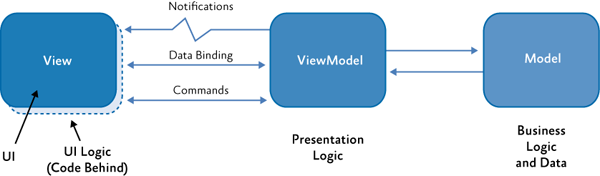
\includegraphics[width=100mm]{Mvvm} 
\caption{Illustrasjon som viser tre MVVM klasser og hvordan interaksjonen mellom dem\cite{Im1online}} 
\label{fig:mvvm} 
\end{figure}


\subsection{Modell}

Modell delen av MVVM står for en av de viktigste delene i enhver applikasjon, nemlig data og informasjon. Modellen sin eneste jobb er å representere og holde dataene som applikasjonen skal bruke. Den skal ikke hente data fra en database eller manipulere data på noen som helst måte \cite{Model7:online}. Dette går under forretningslogikk og skal ifølge mønsteret holdes separat fra modell-klasser. 


\subsection{View}
 
 Som navnet impliserer, skal klasser definert som View stå for visuelle elementer som vinduer, knapper, tekst, farger og organiseringen av dem. Med andre ord, selve brukergrensesnittet \cite{THEM6:online}. Grafiske objektet kan skrives ved hjelp av kode, men i MVVM skal alt som har med View og gjøre skrives XAML.
 
\subsection{ViewModel}
 
 Som en kan se utifra figur \ref{fig:mvvm} ligger Viewmodellen mellom Model og View. Så mens modellen holder data og Viewet presenterer data så er det Viewmodellen sin jobb å manipulere eller håndtere data. Si for eksempel at Modellen holder en dato, disse kan ofte være lagret i et format som ikke er så lettleselig. Det er da ViewModellen sin jobb å konvertere det til et mer leselig format før Viewet presenterer det til leseren. 
 
\subsection{Databinding, Notifikasjon og Kommando}

Et View og en ViewModel skal ifølge mønsteret ha en en-til-en relasjon, der viewet har en referanse til viewmodellen, men ikke omvendt. For at ViewModellen og Viewet skal kunne "snakke" sammen og fortsatt holdes separat brukes databinding, kommandoer og notifikasjoner. 

Viewet presenterer informasjon til brukeren ved å binde seg til egenskaper og kommandoer som Viewmodellen eksponerer, dette kalles for \textbf{databinding}. Når en egenskap endres i ViewModellen vil viewet bli oppmerksom på dette gjennom en notifikasjon og oppdateres deretter. 

En kommando er implementert i ViewModellen, men blir aktivert fra Viewet. Dette skjer ved brukerinput. For eksempel når bruker trykekr eller ser på en knapp.



\subsection{MVVM-light toolkit} 
 
 MVVM-light er et bibliotek som skal hjelpe utviklere med å sette opp MVVM i kodebasen \cite{Nico0:online}. Hensikt ved biblioteket er å akselerere utviklingen av MVVM applikasjoner i WPF, Silverlight, Windows Store, Windows Phone og Xamarin \cite{MVVM8:online}. Dette skal det gjøre ved å levere et utviklingsklart fundament og flere hjelpeklasser. Blant annet så 


Den viktigste grunnen til at dette tredjeparts biblioteket ble tatt med i prosjektet er på grunn av en funksjon kalt DesignTime-Data \cite{MVVMLightDoc:online}. For en av fordelene ved å skrive brukergrensesnittkode i XAML er at en utvikler har mulighet til å se resultatet momentant i et design vindu. Ulempen er at dette kun gjelder for statisk innhold og ikke data som må hentes fra databaser, web-tjenester eller andre kilder. Ved å bruke DesignTime-data kan man bruke en boolsk egenskap som heter IsInDesignModeStatic \cite{MVVM100123:online}. Hvis denne er sann så kan man hente dummy data, hvis ikke så kan det hentes fra den faktiske kilden. Dette gjør at man slipper å kjøre programmet for å se endringer.


\section{Dataformat og lagring}


Programvaren skal strebe etter å kunne tilby de ordene en bruker har lyst å bruke. Noe som kan være utfordrende med tanke på at et barns vokabular allerede i alder av 5 år kan være opp i mot 2000 ord. Hvilke 2000 ord dette er, vil også variere fra person til person noe som øker utfordringen. For vært ord må det også være et symbol som representerer det. En naiv fremgangsmåte ville vært å statisk initialisert hver brikke med et ord og bilde. Problemet med dette er først og fremst at XAML koden blir svært lang, som følge av at en må skrive en knapp for vært tilfelle. Den andre er at en også må inn i koden for å gjøre endringer eller legge til nye ord. Så for å oppbevare skille mellom data og brukergrensesnitt ble all data lagret separat. I koden er det to datastrukturer som holder data. Den ene er 

Løsningen på ble å oppbevare alle ordene i en separat fil for å skille mellom brukergrensesnitt og data. Det ble laget to variasjoner for lagre data - den ene i JavaScript Object Notation(JSON) dokument den andre som et tekstdokument.

\subsection{JSON}

JSON er et lettvekt data-utvekslings format som skal være lett for mennesker å lese og skrive, og det er lett for maskiner å tolke og generere\cite{JSON7:online}. Figur \ref{listing:jsonfile} viser et utdrag fra en av JSON filene som brukes i prototypen. Hver JSON fil består av en liste med JSON objekter som har attributtene Name og Image. Der Name er ordet og image er stien til symbolet. Dette er bare et lite utdrag fra filen og viser kun det som ville tilsvart fire brikker i programvaren.

I dette dokumentet er det første objektet "I" et ord, mens de tre neste er kategorier. Hver kategori består av flere ord. Ordene som tilhører en kategori er lagret i en egen fil i en mappe med samme navn. 

Figur \ref{jsonstructure} viser strukturen på filene, der hver kategori har sin egen mappe. Dette gjør at data hentes "just-in-time". Det vil si at istedenfor at ordene ligger i minnet til enhver tid, så hentes de kun når ved behov. Eksempelvis hvis en bruker trykker på kategorien "Food and Drink" så vil ordene hentes fra "FoodAndDrink.json" i mappen "FoodAndDrink". Noe som sparer på minnet, men som kan forringe kjøretiden. For når det er snakk om så store mengder data som alle ordene ville gitt, er det ikke gunstig å bevare dem i minnet. 


\begin{listing}[ht] 
\inputminted[fontsize=\footnotesize, frame=lines,framesep=2mm,baselinestretch=1.2,bgcolor=lightgray,linenos]{json}{Code/JSONfile.json} 
\caption{Utdrag fra filen som inneholder ord og sti til bilde som representerer det i JSON format} 
\label{listing:jsonfile} 
\end{listing} 
 

 \begin{figure}[ht!] 
\centering 
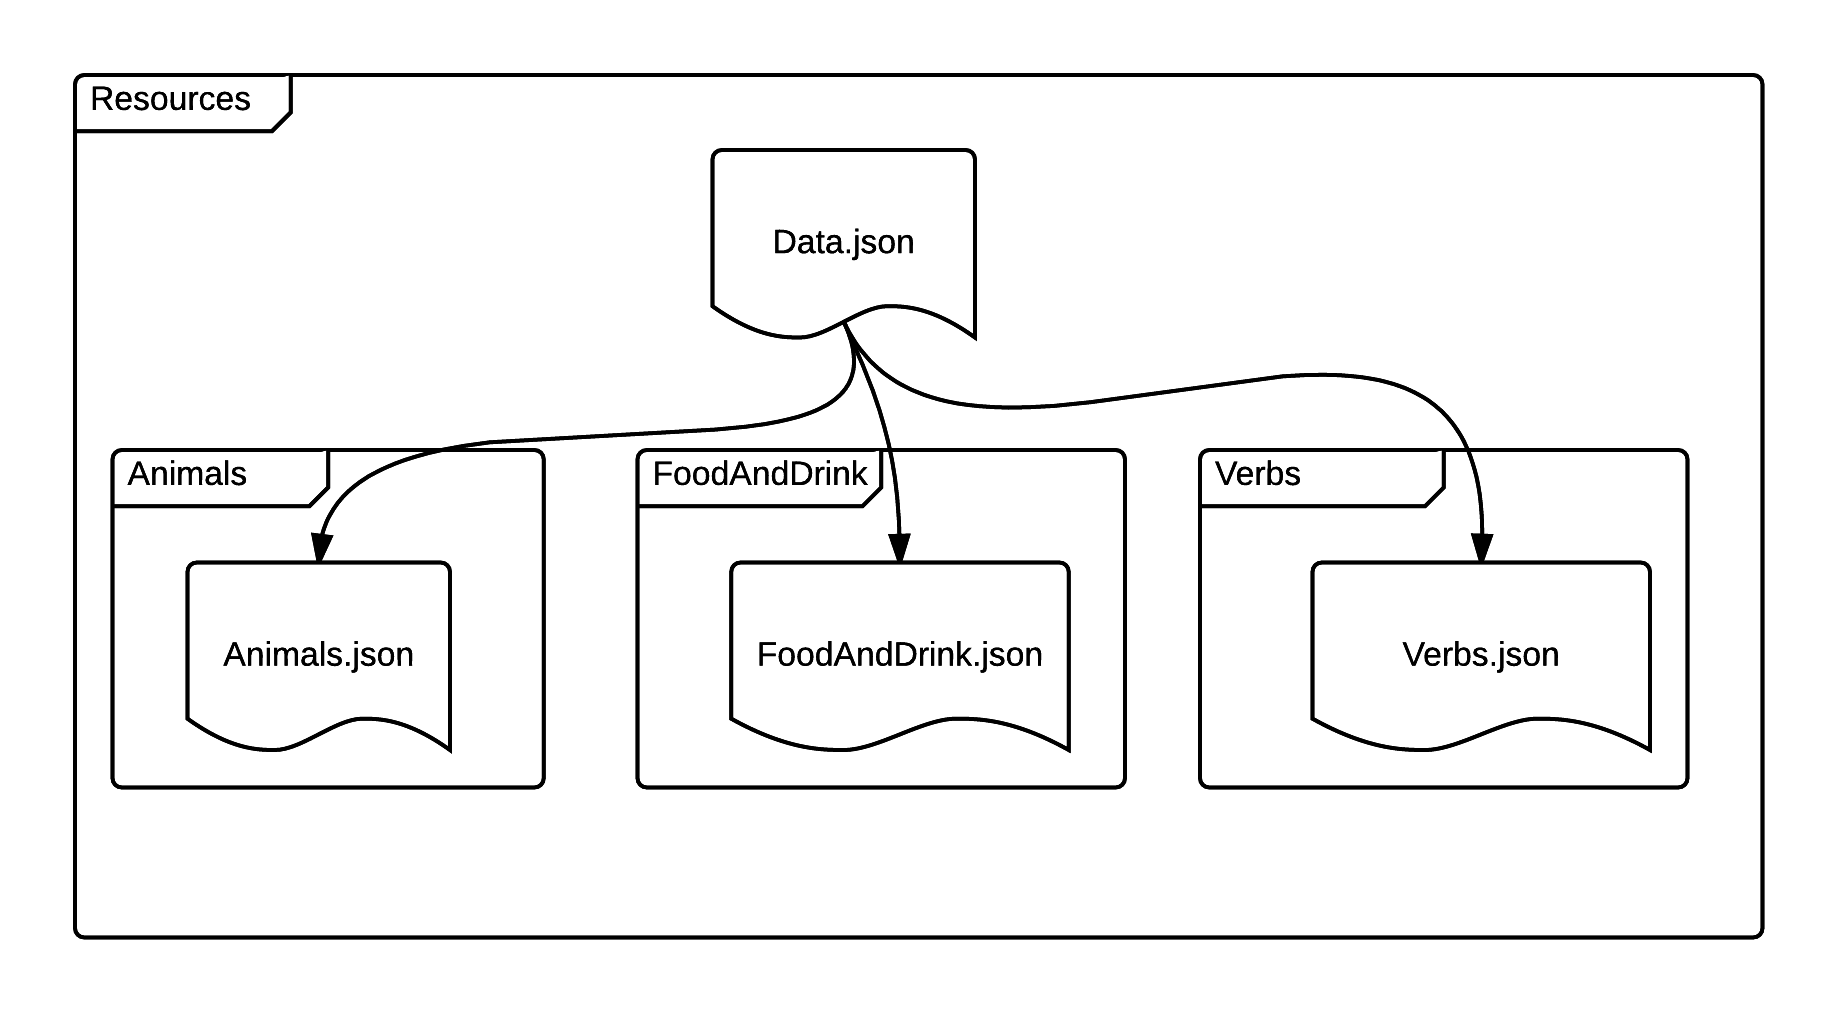
\includegraphics[width=100mm]{JsonStructure} 
\caption{Bilde av dokumentet hvor de ulike symbolene er registrert} 
\label{fig:jsonstructure} 
\end{figure} 


\subsection{JSON-Parsing}

For å kunne ta i bruk objektene definert i tekstfilen må de tolkes fra JSON format til .NET objekter. Denne prosessen, å trekke ut datastrukturer fra bytes, kalles deserialisering. For å gjøre dette har vi brukt et tredjeparts rammevekt kalt JSON.net \cite{Json.0:online}. Det finnes en innebygd funksjon i .NET kalt DataContractJsonSerializer \cite{DataC3:online} som også greier å deserialisere et JSON dokument. Grunnen til at JSON.NET ble brukt er fordi i dette biblioteket er det mulighet å automatisk deserialisere en helt liste av JSON objekter til .NET liste uten å manuelt måtte legge inn objektene. Ifølge utviklerens egne nettsider skal rammeverket være 50 prosent kjappere enn DataContractJsonSerializer, men ytelsen er avhengig av hvilke datasett som brukes, og har ikke vært en faktor i avgjørelsen. 


\begin{listing}[ht] 
\inputminted[fontsize=\footnotesize, frame=lines,framesep=2mm,baselinestretch=1.2,bgcolor=lightgray,linenos]{csharp}{Code/JSONparser.cs} 
\caption{Koden som konverterer JSON filen til en IList} 
\label{listing:JsonParser} 
\end{listing} 


Koden i figur \ref{listing:JsonParser} deserialiserer JSON dokumentet om til en dataliste. Fra linje 5 til 12 skrives teksten fra filen over til en streng som kan manipuleres i koden. På linje nummer 14 blir strengen konvertert til et dataobjekt. Det at dokumentet blir gjort om fra streng til et komplekst objekt på kun en linje viser noe av styrken til json.NET. 


\section{Tekstfil}

Under utviklingen ble det bare lagt inn tilfeldige ord i prototypen, men ettersom prototypen begynte å bli ferdigstilt var det behov for et større utvalg ord og symboler Det ble derfor gitt tillatelse av Tobii Dynavox til å ta i bruk det samme bildene som de bruker i deres programvare. 

\begin{itemize}
\label{itm:egenskaper}
\item Symbol ID
\item Dato oppdatert
\item Dato laget
\item Kategori Navn 
\item Filnavn
\item Filsti
\item Ord
\item Synonymer
\item Tysk, nederlandsk, norsk, svensk, dansk, engelsk, spansk, italiensk, fransk, portugisisk.
\end{itemize}


Sammen med bildepakken fulgte det med et dokument som hadde en beskrivelse av vært symbol. For vært symbol var egenskapene beskrevet i liste \ref{itm:egenskaper} tilgjengelig. Disse var strukturert med at de kom i rekkefølge og hadde tilde notasjon(tilde) for å skille mellom dem. Dette gjorde at det var mulig å implementere en løsning for å gjøre dem om til datastrukturer. I tillegg til å tilby det samme som JSON dokumentet, ord og bildesti, så har den også ordets kategori og synonymer for ordet. Det er også mulighet for å få ordet på flere språk og synonymer til de ulike språkene. Noe som åpnet for flere muligheter, men for å få til dette, måtte det legges til en annen form for innlesing av data ettersom dokumentet ikke var lagret i JSON format og I motsetning til å dele opp symbolene opp i separate dokumenter basert på hvilken kategori de tilhørte, så var alle deklarert på et dokument. Så for å kunne løse dette sto vi mellom å lage et skript som oversatte dokumentet til JSON format eller lage en alternativ innlesning. Å omgjøre det fra tekst til JSON hadde vært mulig, problemet med dette er at dokumentet utsatt for oppdatering. Så hver gang dokumentet blir forandret må oversetting gjøres på ny. Så det ble da bestemt for å implementere en teksttolker. 
\subsection{Teksttolker}

Tekstolkeren er er mer kompleks enn JSON tolkeren. Hovedsaklig fordi det ikke finnes noe bibliotek som automatisk tilegner egenskaper til symbolene. Egenskapene blir derfor gitt til vært symbol etterhvert som de blir lest inn. En annen utfordring var som tidligere nevnt at alt befant seg på et dokument som da totalt utgjorde 16 000 linjer med beskrivelse av symbolene. Slik at hvis en skulle ha brukt samme fremgangsmåte som med JSON parseren å kun lest inn for den gitte kategorien. Så hadde en i verste fall måtte ha lest 16 000 linjer med tekst. Dette er ikke gunstig. Dokumentet har flere kategorier og symboler som ikke er nødvendig for barn, blant annet egne kategorier som eksempel Brasil, hebraisk og sveitsisk. Det er også flere kategorier som kunne vært greit å ha, men som ikke prioriteres som blant annet kategorier om kjendiser og en egen om amerikanske byer. Det ble derfor bestemt å kun velge kategorier som var nødvendige.

\begin{figure}[ht!] 
\centering 
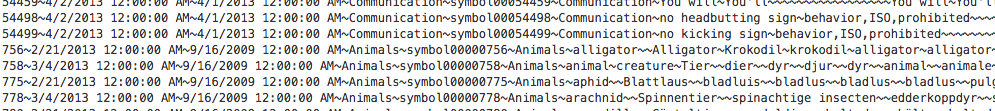
\includegraphics[width=100mm]{datafil} 
\caption{Bilde av dokumentet hvor de ulike symbolene er registrert} 
\label{fig:dok} 
\end{figure} 


\section{Symbol}

Vært objekt i JSON filen og hver linje i tekstfilen blir tolket om til et \textbf{Symbol} objekt. Et symbol sine viktigste egenskaper er Ordet, stien til bilde som representerer ordet og hvilken kategori ordet tilhører. Den har også egenskaper som synonymer, id, forskjellige språk. Figur \ref{fig:symb} er utdrag fra symboltabellen og viser hvordan 4 symboler ser ut i brukergrensesnittet. De to øverste er ord, mens de to på nederste rad representerer kategorier. Symboler som representerer ord vil alltid ha en hvit bakgrunnsfarge med kategorien den tilhører som kant. Kategorier vil alltid ha en annen enn hvit bakgrunnsfarge. Dette er for at det skal være lettere å skille mellom dem.

 \begin{figure}[ht!] 
\centering 
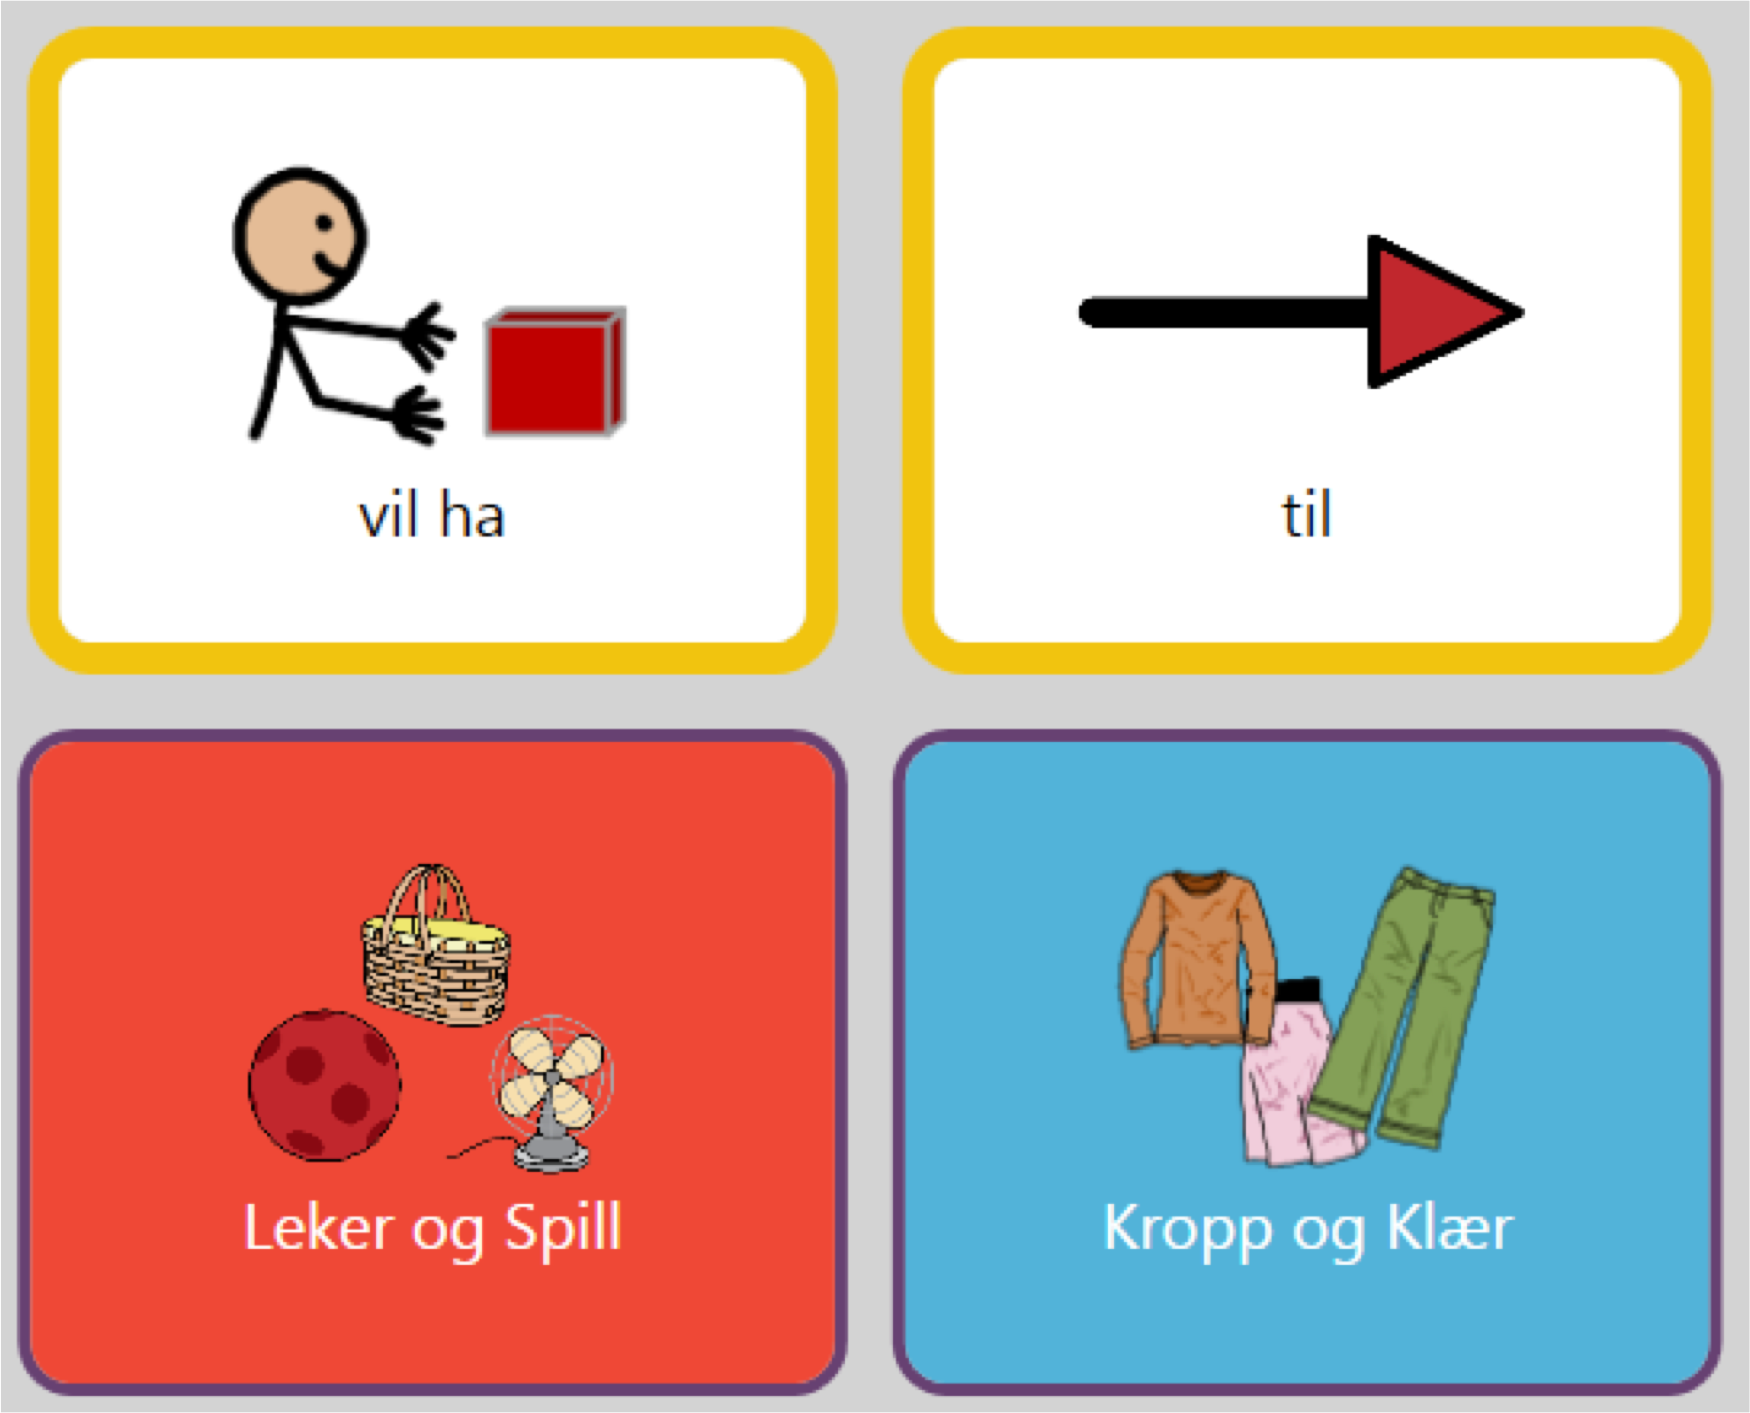
\includegraphics[width=100mm]{Symboler} 
\caption{Fire Symboler vist i brukergrensesnittet} 
\label{fig:symb} 
\end{figure} 

\subsection{SymbolStix}

Bildene som brukes er de samme som i Sono Flex og er kommer fra en bildepakke som heter SymbolStix. Dette er en bildepakke som leveres av et eksternt selskap som heter n2y og har består av rundt 16 000 symboler \cite{n2y}. Grunnen til at disse bildene ble brukt er fordi det ville tatt for lang tid å lage bilder selv eller å finne dem på nettet, som heller ikke er helt lovlig. Disse bildene har fordelen av at de er laget av profosjonelle noe som ses gjennom den gjennomførte stilen og presise tegninger.


\section{Kategori}

Hver kategori har et navn og en liste over alle symbolene som tilhører den. Eksempelvis så vil symbolene med ord som "hest", "ku" og "hund" ligge i listen til kategorien med navnet "dyr". Figur \ref{fig:katego} viser resultatet ved å trykke på kategorien "dyr". 

\begin{figure}[ht!] 
\centering 
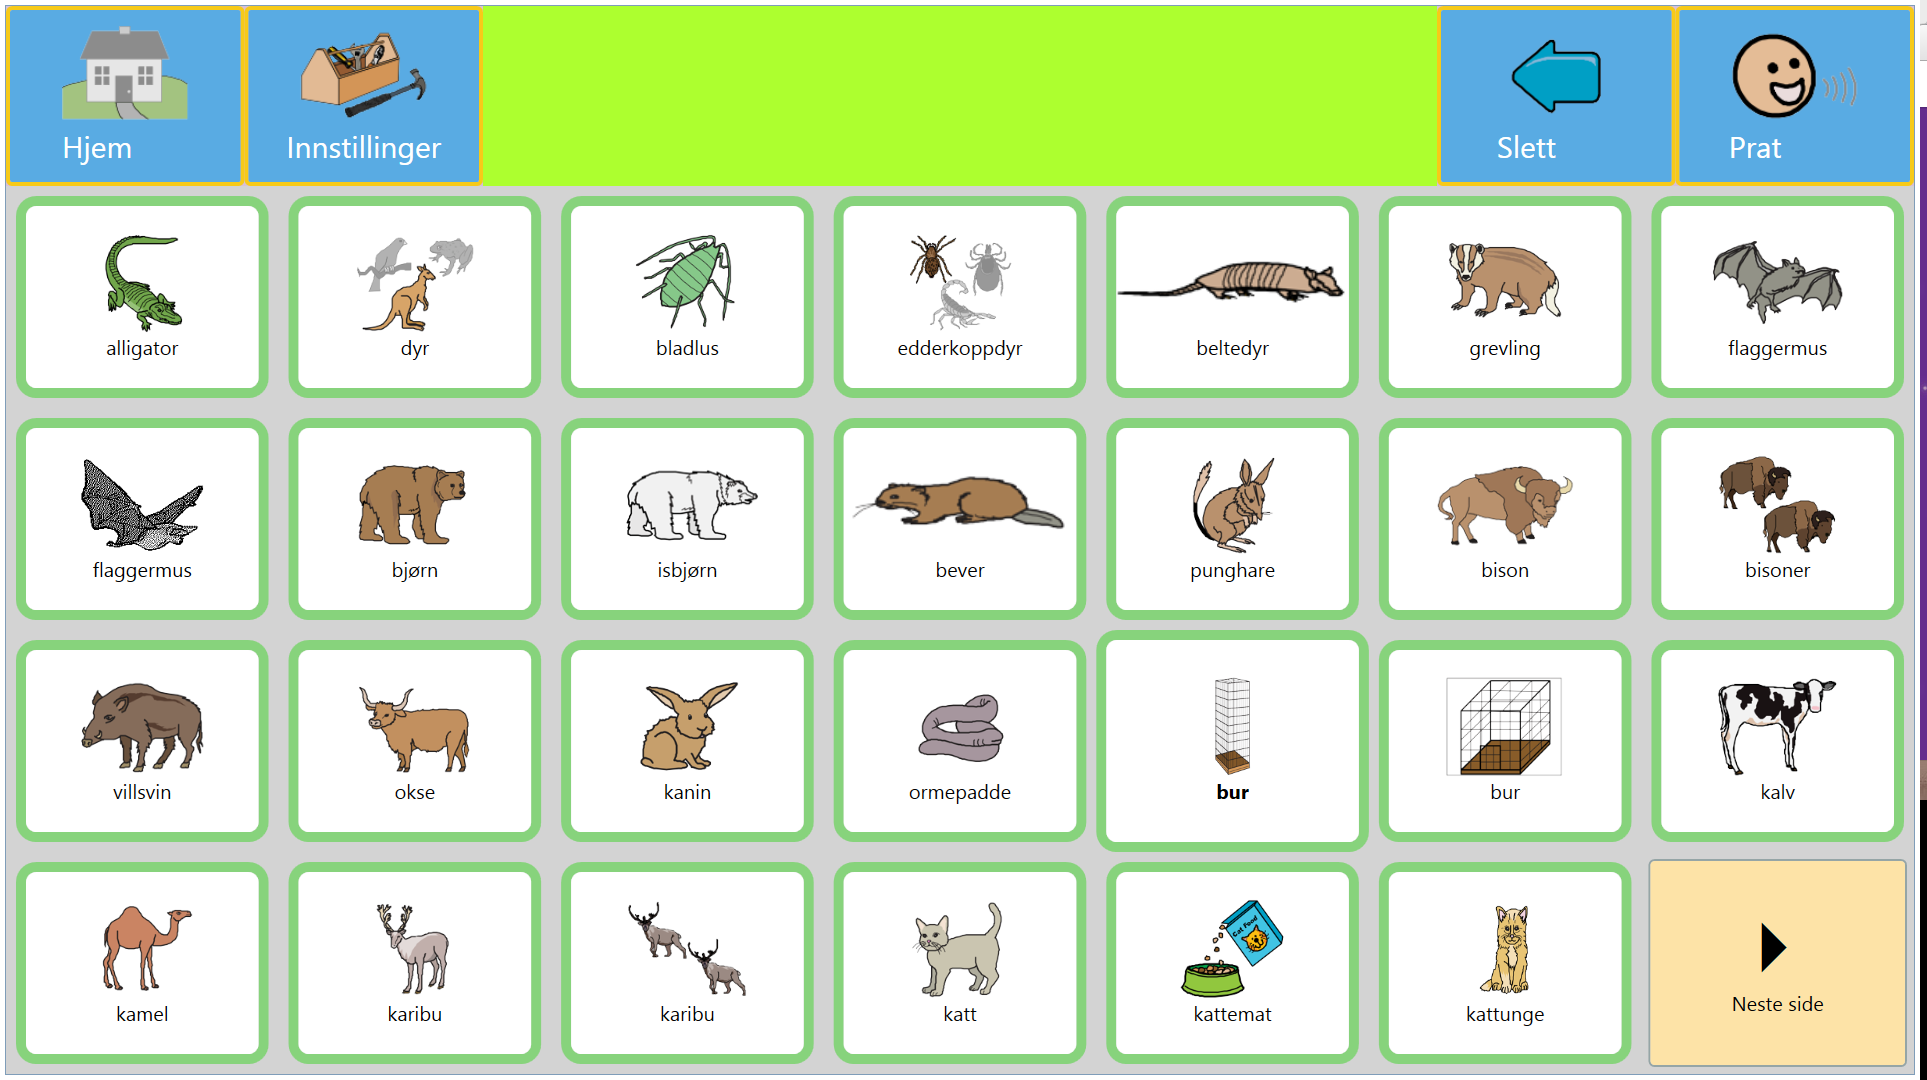
\includegraphics[width=100mm]{dyr} 
\caption{Symbolene på skrivebordet} 
\label{fig:katego} 
\end{figure} 




 
 
\section{Utfordringer}

\subssection{Problem} 
 
Symbolstix bildene er lagret i Enhanced Metafile Fomat (EMF), som er et 32-bit format som kan inneholde både vektor og bitmap informasjon\cite{AboutEMF}. Problemet med EMF formatet er at det ikke finnes støtte for dette i WPF, med den begrunnelse at det har blitt funnet en kritisk sårbarhet\cite{EMFVulnerability} og at formatet er mer mottakelig for sårbarheter\cite{EMFForum} enn andre bildeformater. I Sono Flex fungerer dette fint, fordi det bygget på Windows Forms(WF),  et rammeverk som har innlagt støtte for EMF. WPF har støtte for å bruke WF elementer,  en funksjon som ble lagt inn for å lette overgangen fra WF til WPF. Som igjen gjorde det mulig å hente bilder med EMF format. Ulempen er at man må trekke inn store deler av WF biblioteket noe som fører til en betraktelig økning i størrelse. For å aktivere støtten, deklarerer en WindowsFormHost i xaml filen og denne vil fungere som en kontainer for alle WF elementer. Innenfor denne kontaineren vil alt fungere som i et WF miljø. Ved å gjøre dette ble alle bildene hentes og vist i prototypen.  
 
Testing av applikasjonen viste derimot at det ikke lenger var mulig å trykke på knappene, eller mer korrekt, det var ikke mulig å trykke på  bildet der knappen var. Dette viste seg å være kjent problem, og er kjent som Airspace problemet (kilde) og kommer av at alle WF elementer uansett vil legge seg over alle WPF elementer. Et problem som ikke kunne være med i prototypen. En fix til dette ble laget og planlagt lansert i .NET versjon 4.5, men da versjonen ble lansert, var ikke denne fiksen med. Det finnes ulike omveier rundt på problemet, men få tilfredsstillende.  
 
Det ble derfor prøvd å konvertere EMF filene til bitmap for så å vise de i applikasjonen. Fordelen med denne fremgangsmåten var at vi slapp å trekke inn windows forms biblioteket. Ulempen var derimot at hver gang et symbol skulle hentes så måtte dette først konverteres til Bitmap for deretter og rendres. En tidkrevende prosess som gjorde at det tok flere sekunder å laste brukergrensesnittet. Det ble derfor prøvd å konvertere alle filene og deretter lagre dem som jpg. Konverteringen ville da kun gjøres en gang. Deretter ville applikasjonen hente jpg filene direkte, uten noe omvei. Siden wpf har innebygd støtte for formatet. Igjen viste det seg at dette ikke var godt nok ettersom jpg filene hadde blitt for store i overgangen fra vektor til raster grafikk og de manglet gjennomsiktighet. For mens EMF filene lå på under 10kb endte alle de konverterte filene opp på over 100kb. Noe som i selv ikke er så stort, men som gir utslag på lastingen av applikasjonen når det kan være opp mot 200 bilder som skal lastes. 
 
 
Den endelig løsningen ble å laste ned et profesjonelt konverteringsverktøy kalt AVS Image converter. En svært ømfintlig prosess som tok svært lang tid, men som gjorde det mulig å konvertere de orginale EMF filene til png og samtidig holde størrelsen på rundt 10 kb. 


\subsection{Opplæring}


 
\section{Beskrivelse av prototypen} 

Prototypen har den samme layouten som Tobii Sono Flex, med en menylinje etterfulgt av en symboltabell under. Det er derimot en del variasjoner inne i hver av disse komponentene. 
 
\subsection{Menylinjen} 
 
Menylinjen dekker 1/5 del av applikasjonens vindu og består av 4 knapper og listen over ord som brukeren har trykket på. 
 
\subsubsection{Tilbaketasten} 
 
Tasten som befinner seg til høyre for ordlisten er tilbake tasten. Som på et vanlig tastatur vil et trykk på denne knappen medføre at det siste ordet i ordlisten fjernes. 
 
\subsubsection{Ordlisten} 
 
Når en bruker trykker på et ordsymbol så vil dette legge seg i ordlisten og når han trykker på "prate" knappen så vil ordene i listen bli gitt gjennom høyttalerne som naturlig tale og deretter fjernes fra listen. Selv om det er plass til uendelig med ord i listen så vil det kun være mulig for brukeren å se maks 4 om gangen. Hvis det allerede er fire symboler i listen når brukeren trykker på et nytt symbol, så vil de tre første bli "fjernet" mens det fjerde og det nye symbolet vil være igjen. Hvis brukeren igjen fjerner de to siste ordene ved å trykke på tilbaketasten,  vil ordene som kommer før igjen bli presentert for brukeren i setningslisten.  
 
 
\subsubsection{Hjem} 
Ved å trykke på "hjem" knappen vil brukeren alltid bli ført til førstesiden av applikasjonen uavhengig av hvor han befinner seg.  
 
\subsubsection{Innstillinger} 
Hvis brukeren første er på "hjem" siden av applikasjonen så vil knappen byttes ut med en "innstillinger" knapp. Ved å trykke på denne vil det åpnes et nytt vindu hvor brukeren vil ha mulighet til å sette og endre på diverse innstillinger. Detaljene rundt denne siden er beskrevet i seksjon. 
 
 
\begin{figure}[ht!] 
\centering 
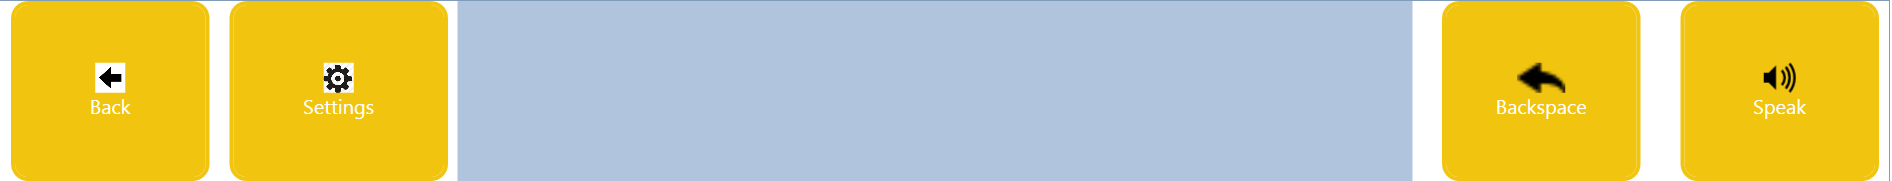
\includegraphics[width=100mm]{MenylinjeP} 
\caption{Skjermdump av menylinjen i prototypen} 
\label{fig:menylinjen} 
\end{figure} 
 
 
\section{Sammendrag} 

Kapittelet forklarer hvordan prototypen fungerer og prosessen med å utvikle den. Prototypen har blitt implementert med en moderne teknologi som fortsatt er støttet. Det har blitt lagt vekt på kodekvalitet under utviklingen. Blant annet så har vi følgt et design mønster som passer bra både til teknologien og plattformen som den skal kjøre på. Alle kravene satt i kravspesifikasjonen har blitt implementert, men noen ikke i like stor grad som ønsket. 

